%%==================================================================%%
%% Author : Tejedo Gonz�lez, Daniel                                 %%
%%          S�nchez Barreiro, Pablo                                 %%
%% Version: 1.0, 27/11/2012                                         %%                   
%%                                                                  %%
%% Memoria del Proyecto Fin de Carrera                              %%
%% Gram�tica, Pruebas                                               %%
%%==================================================================%%

Una vez generados, gracias al uso de EMFText, el editor y el analizador para nuestra gram�tica, procedimos a realizar su correspondiente proceso de pruebas. Para ello escribimos diferentes ficheros de restricciones, probando tanto restricciones correctas como err�neas. Por ejemplo, para el caso de la vinculaci�n de un fichero de restricciones con un �rbol de caracter�sticas, se prob� tanto como rutas correctas como err�neas, absolutas y relativas. 

%%=================================================================%%
%% NOTA(Pablo): Estas figuras se ven fatal, no las metas como      %%
%%              capturas de pantalla o p�salas a EPS mejor         %%
%%=================================================================%%

\begin{figure}[t]
    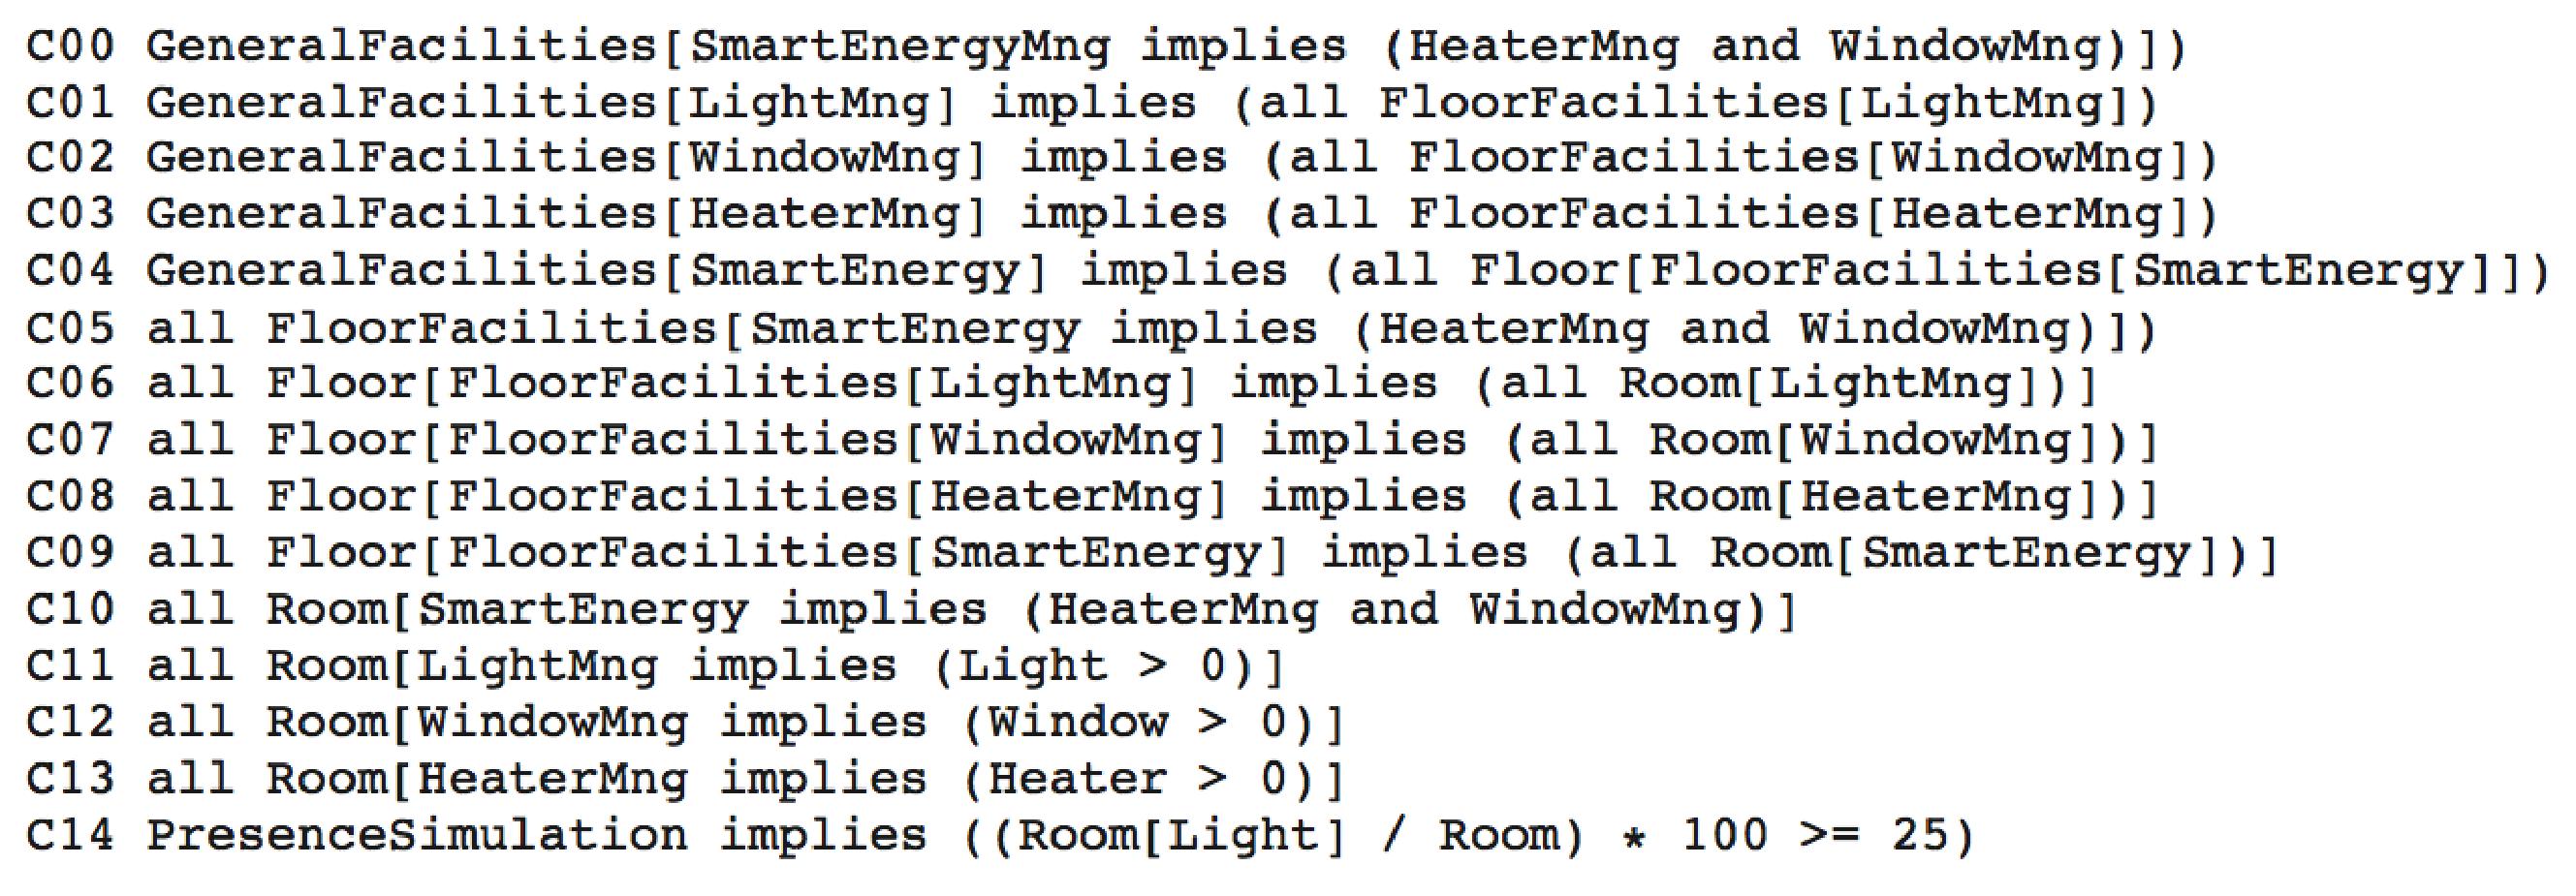
\includegraphics[scale=0.5]{gramatica/oppruebas.eps}
    \caption{Bater�a de instrucciones para probar el funcionamiento de la gram�tica}
    \label{figgrampruebas}
\end{figure}

La Figura~\ref{figgrampruebas} muestra la bater�a de pruebas utilizadas para comprobar el funcionamiento de la gram�tica. Al igual que en los casos anteriores, se trata de un conjunto de pruebas exhaustivas, dise�adas para abarcar todo el conjunto de sentencias que es posible construir con el lenguaje. Tambi�n se analizaron las situaciones excepcionales de sentencias sint�ticamente incorrectas. Para comprobar su correcto funcionamiento, se verific� tanto que el analizador del lenguaje no daba errores al procesarlo, y que el modelo generado como salida del analizador era correcto.

Tambi�n se usaron las instrucciones de las pruebas del cap�tulo anterior, que se pueden observar en la figura \ref{figmetains} para comprobar que el modelo generado era el mismo que el creado manualmente en el cap�tulo anterior.
